\documentclass[10 pt,usenames,dvipsnames, oneside]{article}
\usepackage{../../../modelo-ensino-medio}



\begin{document}

\begin{center}
  \begin{minipage}[l]{3cm}
\includegraphics[width=2cm]{logo}    
\end{minipage}\hfill
\begin{minipage}[r]{.8\textwidth}
 {\Large \scshape Números triagulares no plano}  
\end{minipage}
\end{center}
\vspace{.2cm}

\ifdefined\prof
\begin{objetivos}
\item \textbf{LAF1} Compreender função como uma relação de dependência entre duas variáveis, as ideias de domínio, contradomínio e imagem, e suas representações algébricas e gráficas e utilizá-las para analisar, interpretar e resolver problemas em contextos diversos, inclusive fenômenos naturais, sociais e de outras áreas.
\end{objetivos}

\begin{goals}
\begin{enumerate}

\item[OE1] Representar graficamente.

\end{enumerate}

\tcblower

\begin{itemize}
\item Destaque para os seus alunos que nesse caso não cabe ligar os pontos. As abscissas indicam a ordem sequencial dos números triangulares, portanto, resumem-se apenas a números naturais.

\item Observe que os pontos do gráfico não são colineares.
\end{itemize}

\end{goals}

\bigskip
\begin{center}
{\large \scshape Atividade}
\end{center}
\fi

Represente, no plano cartesiano, o conjunto de pontos que correspondem aos pares ordenados \(\{(n,T_n)\ ;\ n\in\{1,2,...,8\}\}\), em que \(T_n\) é o \(n\)-ésimo número triangular.


\ifdefined\prof
\begin{solucao}

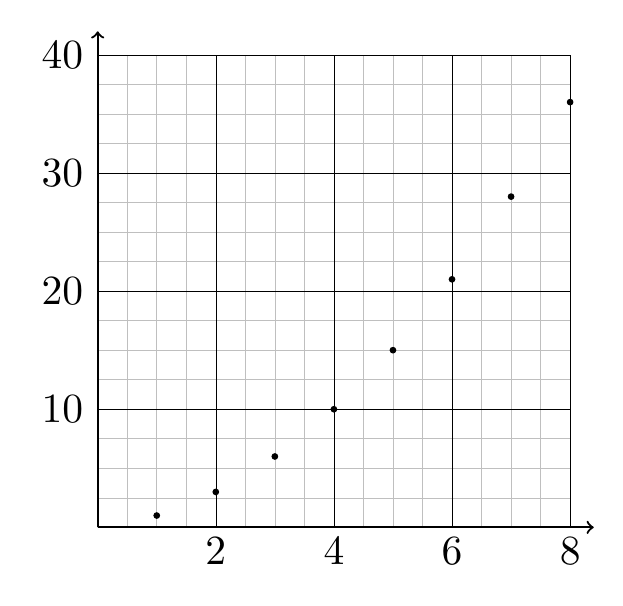
\begin{tikzpicture}[scale=1.5, every node/.style={scale=1.5, black}, every path/.style={color=black}]

\tikzstyle{ponto}=[circle, minimum size=2pt, inner sep=0, draw=black, fill=black, shift only]
\draw[help lines,xstep=.25,ystep=.25, lightgray] (0,0) grid (4,4);
\draw[help lines, black, xstep=1, ystep=1] (0,0) grid (4,4);
\draw[thick,->](0,0)--(4.2,0);
\draw[thick,->](0,0)--(0,4.2);
\foreach \x in {2, 4, 6, 8}
\draw(.5*\x,-.2)node{\x};
\foreach \x in{1, 2, 3, 4, 5, 6, 7, 8}
\node[ponto] at(.5*\x, {.05*\x*(1+\x)}){};
\foreach \y in{10, 20, 30, 40}
\draw(0,.1*\y) node[left]{\y};

\end{tikzpicture}
\end{solucao}
\fi

\end{document}